\documentclass[a4paper,11pt]{article}
\usepackage{polski}
\usepackage[utf8]{inputenc}
\usepackage{graphicx}
\author{Marcin Fabrykowski}
\title{Bezpieczeństwo w sieci. Ochrona sieciowa. Lab 04}
\begin{document}
\maketitle
\newpage
\part{Wstęp}
\section{Co to jest iptables?}
Iptables jest programem pozwalającym na konfiguracje wbudowanego w jądro linuxa filtra pakietów. Iptables służy również do konfigurowania NAT-u.
\subsection{Co to jest NAT?}
Network Address Translation - system translacji adresów sieciowych. Wykorzystywany tam, gdzie nie każdy klient ma swój adres publiczny, a jedynie taki posiada. Pozwala on na komunikację komputerom za natem ze światem. Klienci za NATem posiadają swoje adresy prywatne, niewidoczne dla świata.\\
NAT dzielimy na dwie grupy:
\begin{enumerate}
\item SNAT - Source NAT. Wykorzystywany, gdy chcemy żeby klient mógł połączyć się ze światem, a nie tylko z siecią lokalna. Jest to chyba najczęściej wykorzystywany NAT.\\
Zasada działania: Kiedy klient próbuje wysłać pakiet w świat, wysyła on go z adresem docelowym "światowym" do routera. Tam zostaje zamieniony adres źródłowy z prywatnego klienta, na publiczny routera.
Dzieje się tak dlatego, żeby host docelowy, chcąc odpowiedzieć, mógł skierować odpowiedź do routera który jest widoczny ze świata, a ten dopiero przekaże odpowiedź do klienta. 
\item DNAT - Destination NAT. Rzadziej wykorzystywany. Realizuje on sytuację odwrotną. Gdy jakaś zewnętrzna stacją chce się podłączyć do komputera za NATem, nie ma takiej możliwości bez wykorzystania DNATu. Gdy przychodzi pakiet ze świata na router i zostanie on sklasyfikowany jako pakiet przeznaczony do wnętrza sieci, zostaje podmieniony adres docelowy (routera) na prywatny adres maszyny w sieci i pakiet jest wpuszczany.
\end{enumerate}
\section{Po co jest iptables?}
Iptables pozwala na filtrowanie pakietów przychodzących, wychodzących i przechodzących przez filtrowaną maszynę. Pozwala także na modyfikowanie tych pakietów jak i ich logowanie.
\section{Jak działa iptables?}
Iptables analizuje każdy pakiet który przychodzi do niego. Przepuszczany jest on przez serię tablic. Schemat przejścia pakietu po tablicach, pokazuje rys. \ref{fig:iptables_tablice}.
\begin{figure}
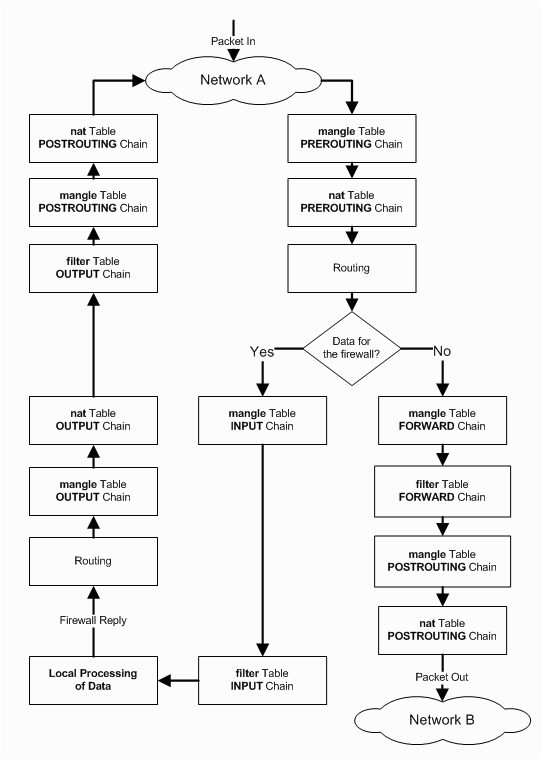
\includegraphics[scale=0.8]{iptables.png}
\caption{Schemat przejścia pakietu po tablicach w iptables}
\label{fig:iptables_tablice}
\end{figure}
\section{Dla kogo jest iptables?}
\begin{enumerate}
\item Z poziomu zwykłego użytkownika, pozwala on zabezpieczyć nasz komputer przed niepożądanymi połączeniami przychodzącymi jak i wychodzącymi.
\item Z punktu widzenia administratora sieci, pozwala na ochronę serwera przed złym światem, jak również na logowanie i filtrowanie ruchu z i do sieci.
\end{enumerate}
\section{Co potrafi iptables?}
\subsection{Rozpoznawanie pakietów}
Iptables potrafi dopasować pakiety wedle wielu różnych kryteriów, m.in.:
\begin{itemize}
\item protoków
\item adres źródłowy
\item adres docelowy
\item interfejs wejściowy
\item interfejs wyjściowy
\item port źródłowy
\item port docelowy
\item flagi TCP
\item typ ICMP
\item mark
\item liczbie pakietów na jednostkę czasu
\item MAC adres
\item TTL
\item dzień,godzina
\end{itemize}
i wiele innych kryteriów pozwalających dokładnie określić, który pakiet należy zaakceptować a który odrzucić
\subsection{Decydowanie o pakiecie}
Po dopasowaniu pakietu, należy zdecydować, co z takim pakietem zrobić. Najpopularniejszymi akcjami jakie można zrobić z pakietami są:
\begin{itemize}
\item zaakceptować
\item odrzucić
\item sklasyfikować
\item DNAT
\item SNAT
\item zalogować
\item zmienić ttl
\end{itemize}
oraz wiele innych
\subsection{Sekwencje wykonywania}
Iptables pozwala na bardziej przejrzyste budowanie firewalla poprzez tworzenie łańcuchów z własnymi sekwencjami akcji.
\subsection{Portknocking}
Jest to sztuczka, polegająca na odrzucaniu pakietów przychodzących na dany port, z możliwością przepuszczania pakietu, jeżeli wcześniej została wysłana specjalna sekwencja pakietów na inne porty, tzw. \textit{pukanie}.
\subsection{Load Balancing}
Inna ciekawą możliwością jest load balancing. Wykonuje się to za pomocą dopasowania \textit{state} oraz wykorzystaniem licznika. Każde nowe połączenie jest kierowane do innego serwera z puli. W efekcie otrzymuje się zrównoważenie obciążenia redundantnych serwerów w sieci.
\subsection{IPset}
Zdarza się, że nasze reguły obejmują sprawdzanie czy np: ip wychodzącego pakietu należy do zarejestrowanego użytkownika czy też do nowo podpiętego. Znając listę adresów ip naszych klientów, moglibyśmy napisać po jednej regule na każdy komputer z odpowiednimi opcjami --src. Jednak takie wyjście jest czasochłonne, zaciemnia firewalla dużą liczba reguł, a dodanie bądź usunięcie klienta, wiąże się z ingerencją w reguły co bywa czasem niebezpieczne.\\
Z pomocą przychodzą ipsety. Pozwalają stworzyć, np: bazę adresów ip naszych klientów, a w firewallu jedynie odwołać się, czy adres źródłowy pakietu znajduje się w danych ipsecie.\\
W takiej sytuacji dodanie bądź usunięcie klienta odbywa się tylko w ipsecie bez zmiany reguł w iptables. Dodatkowo przeszukiwanie ipseta jest wydajniejsze niż sprawdzanie wszystkich reguł w iptables.
\part{Wykonanie ćwiczenia}
\section{Podstawowe polecenia iptables}
\subsection{Blokowanie połączeń wychodzących}
Na początek spróbujemy zablokować połączenia wychodzące. Spróbujmy wejść na stronę: \textit{www.ftj.agh.edu.pl}. Powinna się ona załadować. Następnie wyjdźmy z niej.\\
Teraz spróbujemy zablokować do niej dostęp z naszego komputera. Wykonujemy jako root polecenie:
\begin{verbatim}
iptables -A OUTPUT --dst www.ftj.agh.edu.pl -j DROP
\end{verbatim}
Powyższe polecenie dodaje regułę do łańcucha OUTPUT, czyli tego przez który przechodzi każdy wygenerowany przez nas pakiet. Następnie sprawdza czy adres docelowy pakietu jest równy adresowi w regule, jeśli jest taki sam to dropuje pakiet.\\
Spróbujmy wejść teraz na \textit{www.ftj.agh.edu.pl}. Widzimy, że nie jesteśmy się w stanie połączyć, i wyskakuje timeout. Dzieje się tak dlatego, że przeglądarka wysyła zapytanie, które jest na wyjściu z komputera zapominane i nigdy nie dochodzi do \textit{www.ftj.agh.edu.pl}.\\
\subsection{Podgląd aktualnych reguł}
Przy dłuższym firewallu możemy zapomnieć jakie reguły dodaliśmy do niego. Dlatego pomocną opcją, jest wyświetlenie reguł. Wpiszmy w konsoli:
\begin{verbatim}
iptables -L
iptables -L -v
\end{verbatim}
Oba powyższe polecenia wyświetlą nam aktualne reguły w naszym firewallu dla łańcuchów \textit{INPUT, FORWARD, OUTPUT} dla tablicy \textit{filter}, która jest domyślną i zalecaną tablicą do filtrowania pakietów. Opcja -v dodaje nam statystyki ilościowe i objętościowe pakietów które przeszły przez daną regułę. 
\subsection{Usuwanie reguł}
Ale mu jednak lubimy nasz wydział, i chcielibyśmy móc wchodzić na jego stronę. Musimy więc usunąć blokujący nas wpis. Możemy to zrobić na kilka sposobów:
\begin{enumerate}
\item Możemy podać numer reguły którą chcemy usunąć, np:
\begin{verbatim}
iptables -D OUTPUT 1
\end{verbatim}
co staje się trudne w przypadku większych firewalli.
\item Możemy podać definicje reguły którą chcemy usunąć, czyli skopiować naszą regułę blokującą i zamienić \textit{-A} na \textit{-D}
\begin{verbatim}
iptables -D OUTPUT --dst www.ftj.agh.edu.pl -j DROP
\end{verbatim}
\item Ostatnią, dość brutalną metodą, jest wyczyszczenie całej tablicy reguł. Możemy to zrobić za pomocą:
\begin{verbatim}
iptables -F OUTPUT
\end{verbatim}
\end{enumerate}
\subsection{Polityki}
Jednym z parametrów iptables, są tzw. polityki. Jest to standardowa akcja którą podejmuje firewall w przypadku gdy pakiet przejdzie przez całego firewalla i nie zostanie zdecydowane czy należy go zaakceptować czy odrzucić. Ogólnie przyjętym założeniem jest, że należy wszystko dropować, oprócz żeby które chcemy zaakceptować.\\
Ustawmy politykę \textit{DROP} dla wszystkich połączeń przychodzących:
\begin{verbatim}
iptables -P INPUT DROP
\end{verbatim}
W tej chwili żaden pakiet nie zostanie dopuszczony do naszego komputera. Ale mu lubimy nasz wydział i wierzymy, że nie grozi nam żadne niebezpieczeństwo z jego strony. Możemy wpuścić do nas stronę wydziału:
\begin{verbatim}
iptables -A INPUT -p udp --sport 53 -j ACCEPT
iptables -A INPUT --src www.ftj.agh.edu.pl -j ACCEPT
\end{verbatim}
pierwsza linijka przepuszcza dnsy, które mogą się przydać przy rozwiązywaniu nazw. Druga wpuszcza pakiety przychodzące z \textit{www.ftj.agh.edu.pl}. Spróbujmy teraz wejść na stronę wydziału. A spróbujmy wejść na stronę wydziału.\\
Następnie spróbujmy wejść na inną stronę. O ile ma inne ip, niż strona wydziału, nie uda się jej załadować, gdyż pakiety przychodzące do nas będą odrzucane.
\section{Ciekawsze podstawowe zastosowania}
\subsection{Comment}
Czasami chcemy dodać do firewalla komentarz, że dane pakiety przyszły, np: do statystyk. Możemy to zrobić za pomocą modułu \textit{comment}.
\begin{verbatim}
iptables -A INPUT --src www.google.pl -m comment --comment "Pakiety pochodzace z google.pl"
\end{verbatim}
Każdy pakiet z googla komentujemy. Nie mamy reguły wpuszczającej go do komputera, ale możemy odnotować, że taka próba była. Jest to przydatne przy administracji.
\subsection{Logowanie}
Bardzo często chcemy, aby nasz ruch był logowany w celu wykrywania włamań itp.\\
Robimy to przy pomocy targetu \textit{LOG} oraz opcji \textit{log-prefix}
\begin{verbatim}
iptables -A INPUT -j LOG --log-prefix "polaczenie przychodzace"
\end{verbatim}
w po wykonaniu tego polecenia, wszystkie pakiety przychodzące będą logowane do sysloga. W domyślnej konfiguracji sysloga, będą one zapisywane to \textit{/var/log/messages}
\subsection{Stany połączeń}
W wielu przypadkach, wystarczy rozważyć zaakceptowanie tylko pierwszego pakietu z połączenia, a następnie uznać, że jeżeli puściliśmy pierwszy pakiet, to ufamy temu połączeniu. Możemy skorzystać z możliwości conntracka, który śledzi, czy kolejne pakiety są częścią juz istniejącego połączenia. Jeśli tak, możemy je zaakceptować bez prowadzenia czasochłonnej procedury decydowania o akceptacji pakietu.
Dlatego warto umieścić na początku firewalla poniższą instrukcję:
\begin{verbatim}
iptables -A INPUT -m state --state ESTABLISHED,RELATED -j ACCEPT
\end{verbatim}
Aby sprawdzić jak ona działa, dodajmy jeszcze logowanie. Całość przedstawia poniższy skrypt:
\begin{verbatim}
iptables -F
iptables -A OUTPUT -m state --state ESTABLISHED,RELATED -j ACCEPT
iptables -A OUTPUT -j LOG
\end{verbatim}
Zobaczymy w logach tylko pierwszy pakiet z każdego połączenia które wykonamy. Pozwala to na śledzenie zawiązywanych połączeń, oraz zachowanie przejrzystości i małej objętości logów.
\end{document}
